\documentclass{article}

% if you need to pass options to natbib, use, e.g.:
%     \PassOptionsToPackage{numbers, compress}{natbib}
% before loading neurips_2026

% The authors should use one of these tracks.
% Before accepting by the NeurIPS conference, select one of the options below.
% 0. "default" for submission
% \usepackage{neurips_2026}
% the "default" option is equal to the "main" option, which is used for the Main Track with double-blind reviewing.
% 1. "main" option is used for the Main Track
%  \usepackage[main]{neurips_2026}
% 2. "position" option is used for the Position Paper Track
%  \usepackage[position]{neurips_2026}
% 3. "eandd" option is used for the Evaluations & Datasets Track
 % \usepackage[eandd]{neurips_2026}
% 4. "creativeai" option is used for the Creative AI Track
%  \usepackage[creativeai]{neurips_2026}
% 5. "sglblindworkshop" option is used for the Workshop with single-blind reviewing
 % \usepackage[sglblindworkshop]{neurips_2026}
% 6. "dblblindworkshop" option is used for the Workshop with double-blind reviewing
 \usepackage[dblblindworkshop]{neurips_2026}
% 7. "education" option is used for the Education Track
%  \usepackage[education]{neurips_2026}


% After being accepted, the authors should add "final" behind the track to compile a camera-ready version.
% 1. Main Track
 % \usepackage[main, final]{neurips_2026}
% 2. Position Paper Track
%  \usepackage[position, final]{neurips_2026}
% 3. Evaluations & Datasets Track
 % \usepackage[eandd, final]{neurips_2026}
% 4. Creative AI Track
%  \usepackage[creativeai, final]{neurips_2026}
% 5. Workshop with single-blind reviewing
%  \usepackage[sglblindworkshop, final]{neurips_2026}
% 6. Workshop with double-blind reviewing
%  \usepackage[dblblindworkshop, final]{neurips_2026}
% Note. For the workshop paper template, both \title{} and \workshoptitle{} are required, with the former indicating the paper title shown in the title and the latter indicating the workshop title displayed in the footnote.
% For workshops (5., 6.), the authors should add the name of the workshop, "\workshoptitle" command is used to set the workshop title.
\workshoptitle{AI for Chip Design}
% 7. Education Track
% \usepackage[education, final]{neurips_2026}

% "preprint" option is used for arXiv or other preprint submissions
 % \usepackage[preprint]{neurips_2026}

% to avoid loading the natbib package, add option nonatbib:
%    \usepackage[nonatbib]{neurips_2026}

\usepackage[utf8]{inputenc} % allow utf-8 input
\usepackage[T1]{fontenc}    % use 8-bit T1 fonts
\usepackage{hyperref}       % hyperlinks
\usepackage{url}            % simple URL typesetting
\usepackage{booktabs}       % professional-quality tables
\usepackage{amsmath}        % \text in math mode
\usepackage{amsfonts}       % blackboard math symbols
\usepackage{nicefrac}       % compact symbols for 1/2, etc.
\usepackage{microtype}      % microtypography
\usepackage{xcolor}         % colors
\usepackage{graphicx}       % figures

% Note. For the workshop paper template, both \title{} and \workshoptitle{} are required, with the former indicating the paper title shown in the title and the latter indicating the workshop title displayed in the footnote. 
\title{Understanding representation learning in RL-based logic optimization}


% The \author macro works with any number of authors. There are two commands
% used to separate the names and addresses of multiple authors: \And and \AND.
%
% Using \And between authors leaves it to LaTeX to determine where to break the
% lines. Using \AND forces a line break at that point. So, if LaTeX puts 3 of 4
% authors names on the first line, and the last on the second line, try using
% \AND instead of \And before the third author name.


\author{%
  David S.~Hippocampus\thanks{Use footnote for providing further information
    about author (webpage, alternative address)---\emph{not} for acknowledging
    funding agencies.} \\
  Department of Computer Science\\
  Cranberry-Lemon University\\
  Pittsburgh, PA 15213 \\
  \texttt{hippo@cs.cranberry-lemon.edu} \\
  % examples of more authors
  % \And
  % Coauthor \\
  % Affiliation \\
  % Address \\
  % \texttt{email} \\
  % \AND
  % Coauthor \\
  % Affiliation \\
  % Address \\
  % \texttt{email} \\
  % \And
  % Coauthor \\
  % Affiliation \\
  % Address \\
  % \texttt{email} \\
  % \And
  % Coauthor \\
  % Affiliation \\
  % Address \\
  % \texttt{email} \\
}


\begin{document}


\maketitle


\begin{abstract}
  Computer chips ought to be as small as possible for cost efficiency. The problem of minimizing chip size while preserving the chip's functionality has been studied through the prism of and-inverter graphs (AIGs) since any boolean function can be represented by AIGs.
  Because the complexity of AIG size minimization is unkown (it is NP-hard under some assumptions), it is a fitting candidate for neural solvers that can leverage learned representations to generalize to unseen AIGs and outpace standard enumerations and branch-and-bound solvers.
  Reinforcement learning and more generally planning have been used to optimize such AIGs without the need for intractable supervision signals. Contemporarily, graph representation learning have been applied to train models that can perform tasks on unseen AIGs.
  More recently, those two technologies have been combined and achieved competitive performances with state-of-the-art heuristics.
  In this preliminary work, we question the adequacy of graph representation learning to improve deep reinforcement learning for logic AIG minimization.
\end{abstract}



\section{Introduction}
\paragraph{Contributions:} First, we show that when replicating past work's graph reinforcement learning pipelines, grah representation learning did not help the training compared to simple multi-layer parceptrons trained with graphs statistics (number of nodes, edges, \dots). More fundamentally, we show that both theoretically and empiricially many graph representations, even AIG-specific ones, cannot predict the values of AIGs--in the RL sense--more accurately than standard multi-layer perceptrons trained on graphs statistics only.


\section{Related work}
\subsection{Combinational optimization}
\subsection{Graph represntation learning for AIGs} (GraphBench, DeepGate, \dots)
\subsection{Reinforcement learning for AIGs} (AlphaSynth, MLCAD, \dots)
\subsection{Graph reinforcement learning for other combinatorial optimization} (review paper \dots)

\section{Background material}
\subsection{And-inverter graphs minimization}
\subsection{Markov decision process}

\section{Methodology}
\subsection{Graph state representation}
\subsubsection{Graph convolutional networks}
\subsubsection{Engineered graph features}
\subsection{Reinforcement learning}

\section{Experiments}
\subsection{Graph reinforcement learning}

\begin{figure}[t]
  \centering
  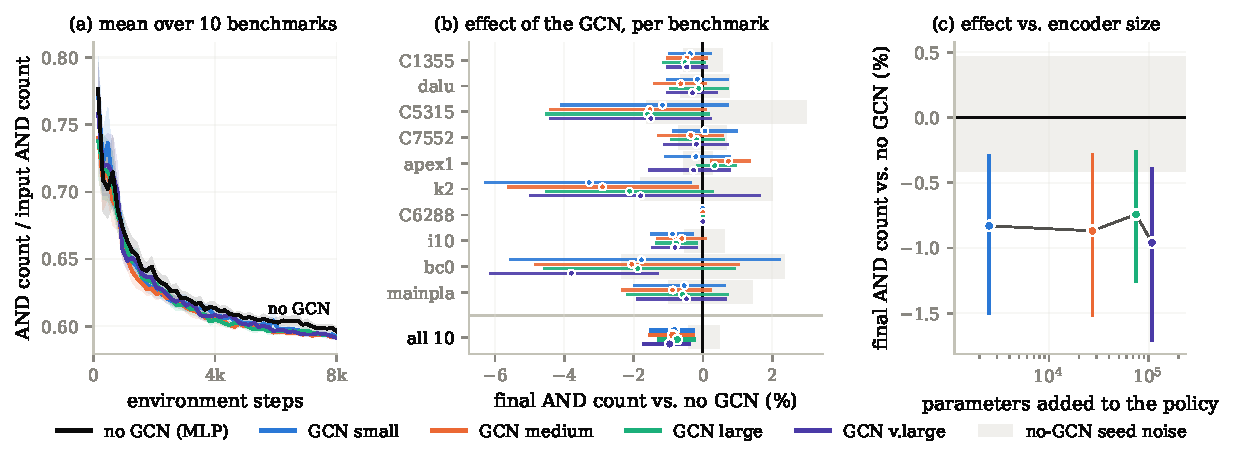
\includegraphics[width=\linewidth]{figures/fig_gcn_main.pdf}
  \caption{PPO on the ten MLCAD benchmarks with five observation encoders,
  hyper-parameter matched. (a) mean AND count over the ten benchmarks;
  (b) per-benchmark change against the MLP, shaded band is one seed standard
  deviation; (c) mean reduction against the parameters the encoder adds to the
  policy.}
  \label{fig:rl-main}
\end{figure}

\begin{figure}[t]
  \centering
  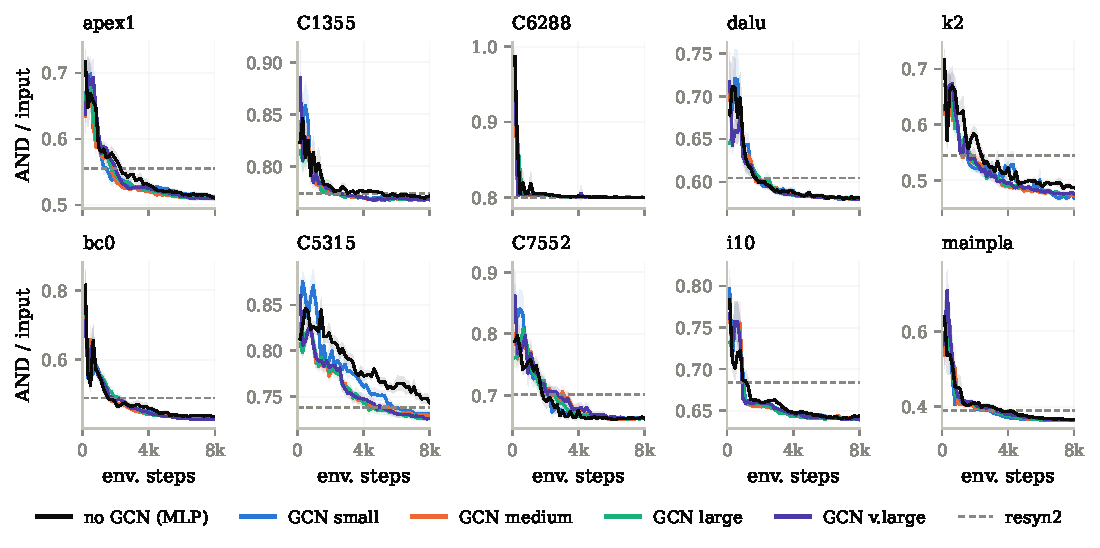
\includegraphics[width=\linewidth]{figures/fig_gcn_per_benchmark.pdf}
  \caption{Per-benchmark learning curves for the runs aggregated in
  Figure~\ref{fig:rl-main}(a). Dashed line: \texttt{resyn2}.}
  \label{fig:rl-per-benchmark}
\end{figure}

\paragraph{Adding a GCN to the policy does not improve AIG minimization
(Figures~\ref{fig:rl-main},~\ref{fig:rl-per-benchmark}).}
We train PPO on ten MLCAD benchmarks with five observation encoders --- an MLP
on graph statistics and four GCNs spanning $2{,}496$ to $107{,}968$ added
parameters --- over a grid of three learning rates, three entropy coefficients
and five seeds, for $2{,}250$ runs in total. Encoders are compared only on the
$424$ of $450$ (benchmark, learning rate, entropy, seed) cells that all five
completed, so no encoder is tuned against the others. Every GCN reduces the
final AND count by $0.76$--$0.85\%$ relative to the MLP, which is less than the
$1.23\%$ standard deviation induced by changing the seed alone, and a $43\times$
increase in encoder size moves that figure by nothing.

\begin{figure}[t]
  \centering
  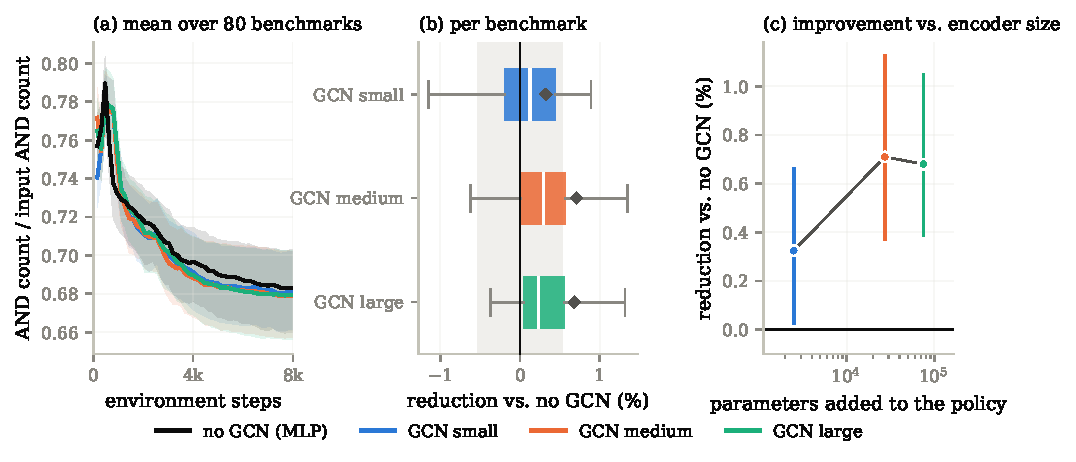
\includegraphics[width=\linewidth]{figures/fig_gcn_ex_main.pdf}
  \caption{The same comparison on \texttt{ex200}--\texttt{ex299}, where each
  encoder ran at its own baseline hyper-parameters. Restricted to the $390$ of
  $500$ (benchmark, seed) cells all four encoders completed, covering $80$
  benchmarks.}
  \label{fig:rl-ex}
\end{figure}

\begin{figure}[t]
  \centering
  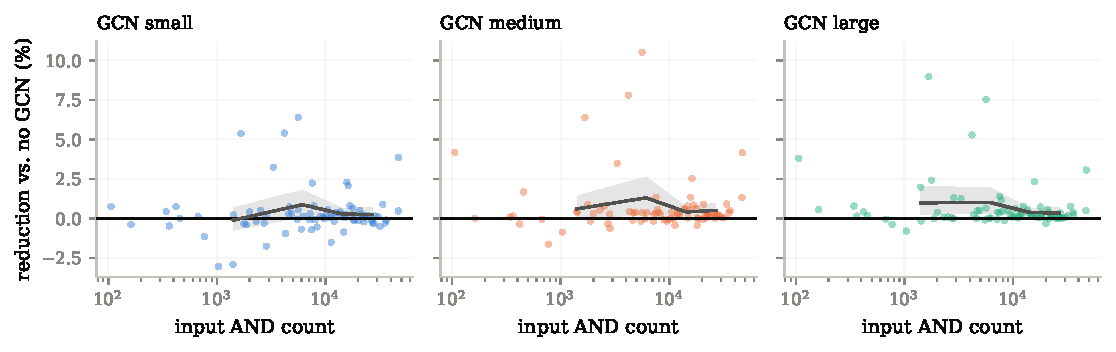
\includegraphics[width=\linewidth]{figures/fig_gcn_ex_size.pdf}
  \caption{Reduction against the MLP as a function of input circuit size on
  \texttt{ex200}--\texttt{ex299}. Line: mean over size quartiles.}
  \label{fig:rl-ex-size}
\end{figure}

\paragraph{The result holds over a hundred further circuits and does not grow
with circuit size (Figures~\ref{fig:rl-ex},~\ref{fig:rl-ex-size}).}
We repeat the comparison on \texttt{ex200}--\texttt{ex299}, a suite spanning
$106$ to $46{,}977$ input AND gates. The three GCNs reduce the final AND count
by $0.33$--$0.71\%$ against a reseed standard deviation of $0.54\%$, and the
effect is flat across two and a half orders of magnitude of circuit size. We
note that the MLP runs were executed on CPU and did not finish on the largest
circuits, which is why $20$ benchmarks are excluded.

\subsection{Value prediction}
\subsubsection{Building a dataset}
\subsubsection{Theoretical lower bounds on the prediction error}

\begin{figure}[t]
  \centering
  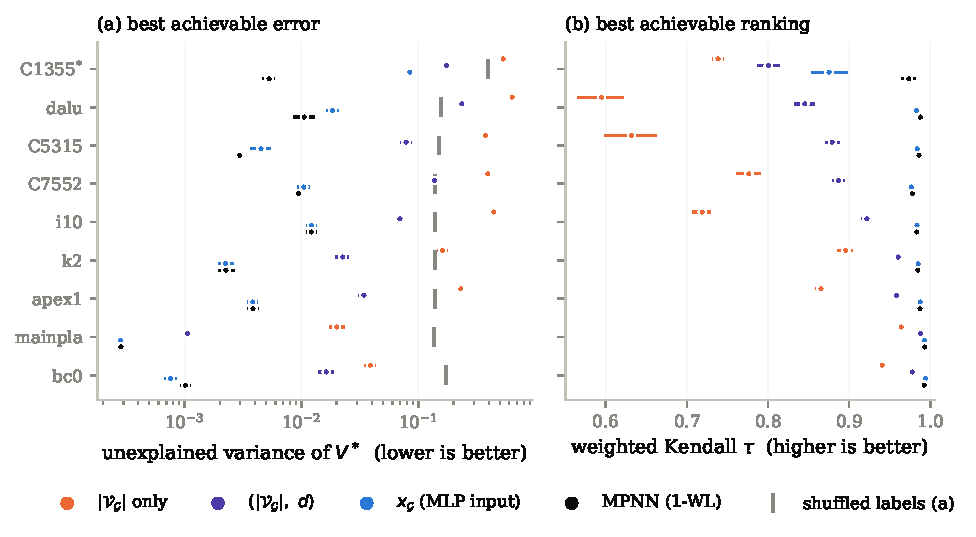
\includegraphics[width=\linewidth]{figures/fig_value_bounds.pdf}
  \caption{Best error (a) and best ranking (b) achievable by each model class on
  $V^\star$, over nine benchmarks and ten dataset seeds. Each class is replaced
  by the optimal predictor for the information it can distinguish, so the value
  shown cannot be beaten by any model in that class. $^{*}$\texttt{C1355} has
  only six distinct targets.}
  \label{fig:bounds}
\end{figure}

\begin{figure}[t]
  \centering
  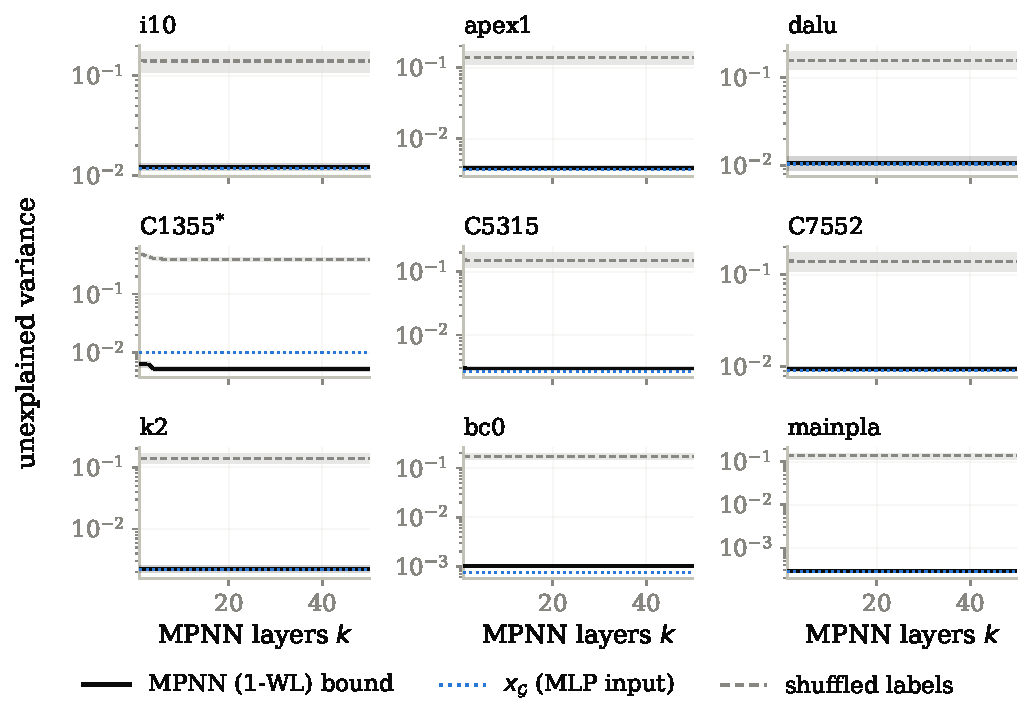
\includegraphics[width=\linewidth]{figures/fig_mpnn_depth.pdf}
  \caption{The MPNN bound as a function of depth $k$.}
  \label{fig:depth}
\end{figure}

\paragraph{Message passing cannot predict $V^\star$ better than the statistics
the MLP already sees (Figures~\ref{fig:bounds},~\ref{fig:depth}).}
A $k$-layer MPNN separates graphs at most as finely as $k$ iterations of
$1$-WL, so grouping states by their $1$-WL colour and predicting each group's
mean $V^\star$ gives an error no MPNN can beat; the same construction bounds a
$0$-layer network, a $(\text{size},\text{depth})$ model, and a model seeing only
the MLP's features $x_\mathcal{G}$. Message passing is worth a great deal over
size and depth alone, but the MLP's own features close almost all of that gap:
the two bounds are within a factor of $1.7$ on eight of nine benchmarks and
within $1.1$ on five, and rank states equally well ($\tau \approx 0.98$).
Depth is irrelevant --- the bound moves by at most $1.1\times10^{-3}$ between
$k=1$ and $k=50$, and edge direction and inverter bits change it by less than
$10^{-6}$. \texttt{C6288} is excluded: its target takes two distinct values.

\subsubsection{Empirical performances of AIG-specific models on value prediction}

\begin{figure}[t]
  \centering
  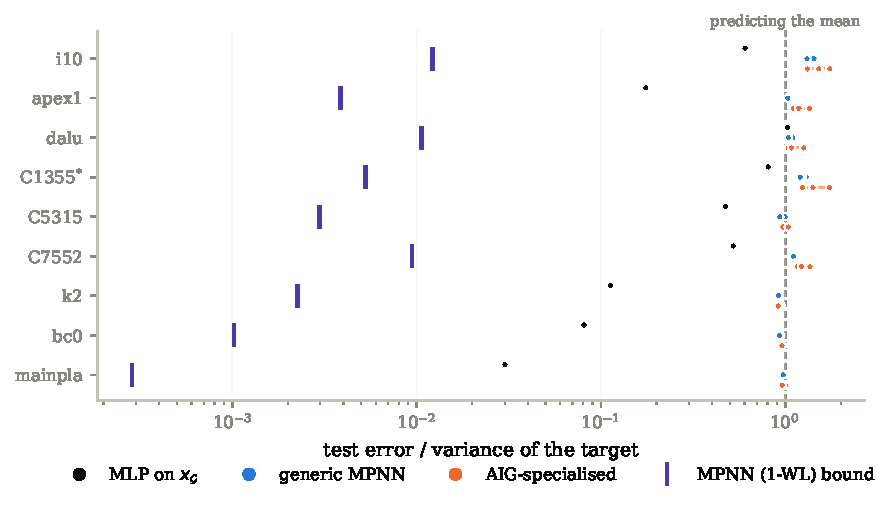
\includegraphics[width=0.92\linewidth]{figures/fig_trained_models.pdf}
  \caption{Test error of eight trained models, normalised by the variance of the
  target so that $1.0$ is the error of predicting the mean. Violet ticks: the
  $1$-WL bound of Figure~\ref{fig:bounds}.}
  \label{fig:trained}
\end{figure}

\begin{figure}[t]
  \centering
  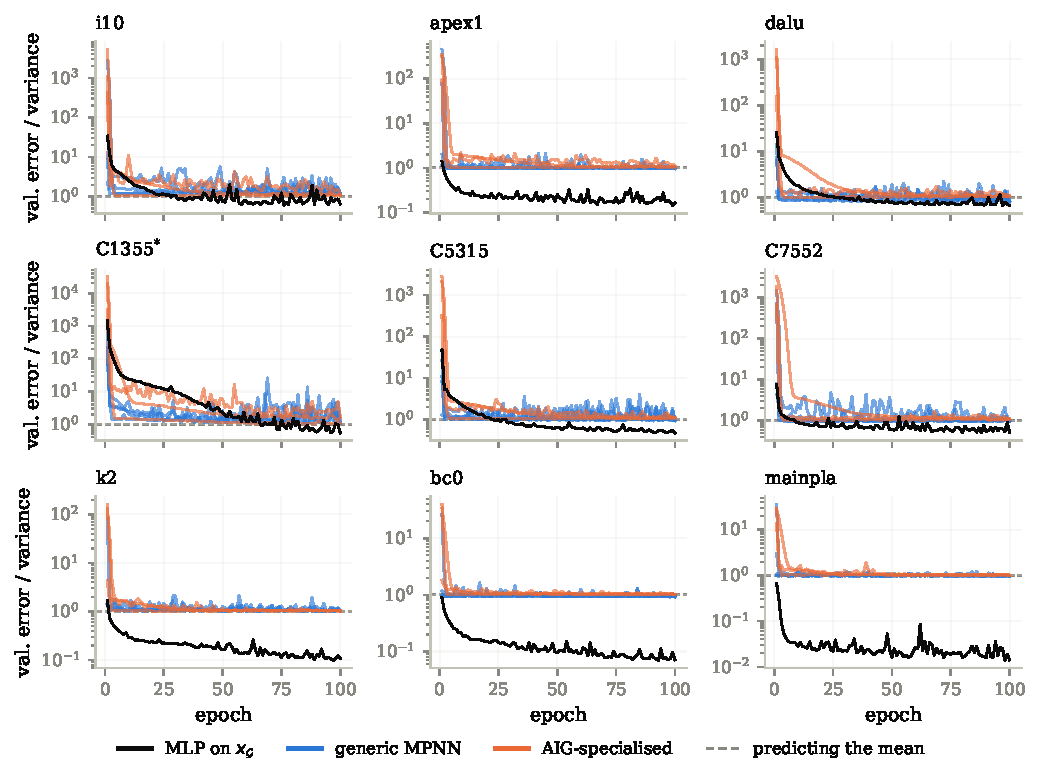
\includegraphics[width=\linewidth]{figures/fig_training_curves.pdf}
  \caption{Validation error over training for the configurations of
  Figure~\ref{fig:trained}.}
  \label{fig:curves}
\end{figure}

\paragraph{Trained graph models, including AIG-specific ones, do not beat
predicting the mean (Figures~\ref{fig:trained},~\ref{fig:curves}).}
We train four generic message-passing networks (GCN, GIN, GAT, GraphSAGE),
three AIG-specific ones (DeepGate, PolarGate, FuncGNN) and an MLP on
$x_\mathcal{G}$, each over its own grid of $36$ configurations ($12$ for
DeepGate), selecting on validation error and reporting test error. All seven
graph models land between $0.90$ and $1.74$ times the target variance --- at or
above the constant predictor --- while the MLP reaches $0.47$ at the median.
Their training error is also $\approx 1$, so this is a failure to fit rather
than to generalise, and it leaves them two to three orders of magnitude above
the bound of Figure~\ref{fig:bounds} that their own architecture class admits.

\section{Futre work}
Many actions


\section*{References}


References follow the acknowledgments in the camera-ready paper. Use unnumbered first-level heading for
the references. Any choice of citation style is acceptable as long as you are
consistent. It is permissible to reduce the font size to \verb+small+ (9 point)
when listing the references.
Note that the Reference section does not count towards the page limit.
\medskip


{
\small


[1] Alexander, J.A.\ \& Mozer, M.C.\ (1995) Template-based algorithms for
connectionist rule extraction. In G.\ Tesauro, D.S.\ Touretzky and T.K.\ Leen
(eds.), {\it Advances in Neural Information Processing Systems 7},
pp.\ 609--616. Cambridge, MA: MIT Press.


[2] Bower, J.M.\ \& Beeman, D.\ (1995) {\it The Book of GENESIS: Exploring
  Realistic Neural Models with the GEneral NEural SImulation System.}  New York:
TELOS/Springer--Verlag.


[3] Hasselmo, M.E., Schnell, E.\ \& Barkai, E.\ (1995) Dynamics of learning and
recall at excitatory recurrent synapses and cholinergic modulation in rat
hippocampal region CA3. {\it Journal of Neuroscience} {\bf 15}(7):5249-5262.
}


%%%%%%%%%%%%%%%%%%%%%%%%%%%%%%%%%%%%%%%%%%%%%%%%%%%%%%%%%%%%

\appendix

\section{Technical appendices and supplementary material}
Technical appendices with additional results, figures, graphs, and proofs may be submitted with the paper submission before the full submission deadline (see above). You can upload a ZIP file for videos or code, but do not upload a separate PDF file for the appendix. There is no page limit for the technical appendices. 

Note: Think of the appendix as ``optional reading'' for reviewers. The paper must be able to stand alone without the appendix; for example, adding critical experiments that support the main claims to an appendix is inappropriate. 

%%%%%%%%%%%%%%%%%%%%%%%%%%%%%%%%%%%%%%%%%%%%%%%%%%%%%%%%%%%%

\newpage
\input{checklist.tex}


\end{document}